%- %%%%

\chapter{Introduzione}

%%%%

\section{Descrizione}
Recenti sviluppi nel trattamento mirato di questo gruppo di malattie fa affidamento sull'accurata inferenza della progressione e dell'evoluzione del cancro \cite{Ciccolella268243}, rivelandosi una . Il cancro è la seconda causa più comune di morte \cite{worldindatacancer}, arrivando nel 2017 a contare il 17.08\% delle morti nel mondo, per un totale di 8.93 \textit{milioni} di decessi.

%%%%

\section{Storia}

Era il 1869 quando venne isolato per la prima volta nella storia dell'umanità l'\textit{Acido Desossiribonucleico}, anche conosciuto come \textit{DNA}. Il pioniere di questa scoperta è Friedrich Miescher, medico e ricercatore nato in Svizzera nel 1844. Durante il processo di scoperta, Miescher aveva realizzato che nonostante  avesse proprietà simili alle proteine, la nuova sostanza -- il DNA -- non lo era. Prima di isolare le cellule dal pus presente nelle bende chirurgiche dell'ospedale in cui lavorava, Miescher fu molto attento ad assicurarsi che il materiale che stava utilizzando fosse fresco e non contaminato. Fu solo più tardi, nel 1871, che il ricercatore iniziò a lavorare sullo sperma di salmone, una specie di pesce che affluiva numerosa durante il periodo autunnale nella città di Basel.

%%%%

\section{Nozioni di biologia}

In questa sezione verranno introdotte nozioni inerenti al lavoro svolto, al fine di poter agevolarne la replicazione e la comprensione.

\subsection{La cellula}

Le cellule costituiscono le fondamenta di tutti gli organismi viventi. Il corpo umano è composto da trilioni di cellule. Esse danno forma al corpo, estraggono le sostanze nutritive dal cibo, convertono quelle sostanze nutritive in energia, ed hanno delle funzioni specifiche. Le cellule contengono anche il materiale ereditario del corpo, e possono fare copie di loro stesse \cite{Whatisac86:online}. Esse sono a loro volta costituite da diverse parti, tra le quali analizzeremo il nucleo e ciò che esso contiene, il DNA.

\subsection{Il DNA}

\begin{wrapfigure}{r}{0.5 \textwidth}
    \centering
    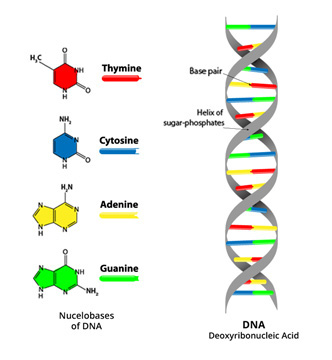
\includegraphics[width=0.75 \linewidth]{./Images/1_dna.jpg}
    \caption{Il DNA}
    \label{fig:dna}
\end{wrapfigure}

Il \textit{DNA}, o \textit{acido desossiribonucleico}, è il materiale erediratio negli umani e quasi tutti gli altri organismi viventi. Quasi ogni cellula presente all'interno del corpo umano ha lo stesso identico DNA. La maggior parte del DNA è situata all'interno del nucleo della cellula (dove è chiamato \textit{DNA cellulare}), ma può trovarsi anche all'interno dei mitocondri, organi cellulari addetti alla respirazione cellulare. Le informazioni nel DNA sono conservate come un codice formato da quattro componenti chimici base (anche dette basi azotate): \textbf{adenina} (A), \textbf{guanina} (G), \textbf{citosina} (C), e timina (T). L'ordine, o la sequenza, di queste basi determina le informazioni disponibili per costruire e mantenere operativo un organismo.

Le basi del DNA si combinano tra di loro, A con T e C con G, in maniera tale da formare unità chiamate \textit{coppie base}. Assieme ad una molecola di zucchero ed una di fosfato, le basi costituiscono quello che è definito un \textit{nucleotide}. I nucleotidi sono disposti in due lunghi fili che formano una spirale chiamata \textit{doppia elica}.

Un'importante proprietà del DNA è che si può replicare, o fare copie di se stesso. Uno qualunque dei due fili di DNA \cite{WhatisDN79:online} può essere utilizzato nel processo di duplicazione per ottenere una copia identica del DNA di partenza. Questa è una fase cruciale nella divisione di una cellula, poiché la nuova copia di essa deve avere lo stesso identico DNA della cellula di origine.

\subsection{Cancro e tumore}

\begin{figure}[h]
    \begin{minipage}{.5 \textwidth}
        \centering
        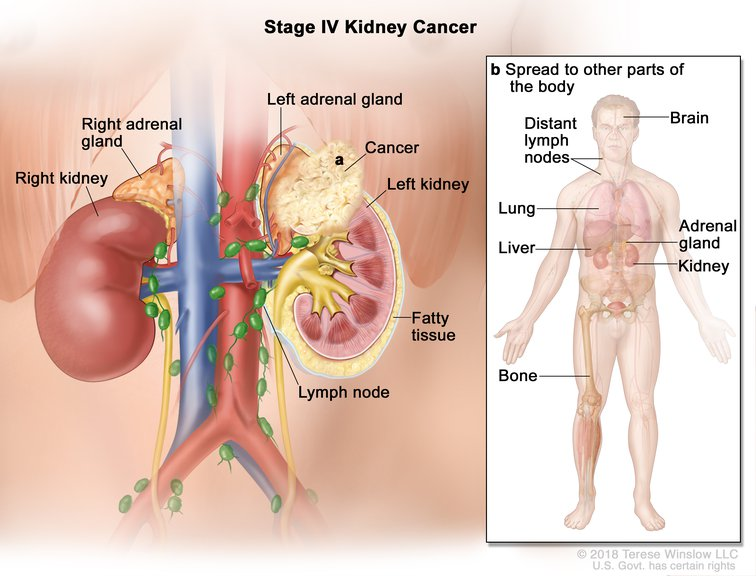
\includegraphics[width=0.75 \textwidth]{Images/1_tumor.jpg}
        \caption{\small Cancro al rene}
        \label{fig:kidney-cancer}
    \end{minipage}%
    \begin{minipage}{.5 \textwidth}
        \centering
        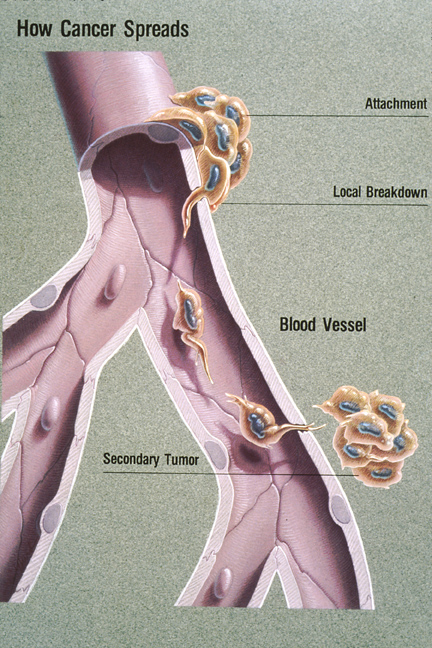
\includegraphics[width=0.35 \textwidth]{./Images/1_metastasi_spread.jpg}
        \caption{\small Diffusione del cancro}
        \label{fig:metastasi}
    \end{minipage}
\end{figure}

La fase di divisione di una cellula è cruciale. Si stima che durante la replicazione, solo una base su $10^9$ \cite{DNAReplication} sia errata. Vari fattori possono inoltre influenzare questa delicata fase, come l'esposizione ad agenti chimici ed irradiazione. Questi errori molto spesso sono corretti in vari modi, ma quando questo non basta, possono essere la causa scatenante che porta una cellula a diventare \textit{cancerogena}. In generale, una cellula è cancerogena quando inizia a moltiplicarsi senza controllo. Quando questo processo avviene in un tessuto solido come un organo (Figura \ref{fig:kidney-cancer}), muscolo od ossa, prende il nome di \textit{tumore}. Ci sono due tipi di tumore: \textit{maligno} (cancerogeno) e \textit{benigno} (non cancerogeno). I primi possono invadere i tessuti circostanti nel corpo, e mentre crescono, alcune cellule possono viaggiare attraverso il sangue (Figura \ref{fig:metastasi}) o altri mezzi a formare delle \textit{metastasi}, dei tumori secondari \cite{differencecancertumor:online}, mentre gli ultimi conservano le caratteristiche del tessuto di origine e non hanno la tendenza di invadere gliorgani circostanti. Un tumore benigno non è quindi un cancro, ma solo una massa che può raggiungere dimensioni considerevoli, ma non si diffonde in altre parti del corpo.